\documentclass[ignoreonframetext,unicode]{beamer}

\usepackage[utf8]{inputenc}
\usepackage[T1]{fontenc}
\usepackage[english,russian]{babel}
\usepackage{amsmath}
\usepackage{amsfonts}
\usepackage{amssymb}
\usepackage{graphicx,pgf}
\usepackage{multimedia}

\usetheme{Warsaw}

\useinnertheme{circles}   %внутренняя тема
%\useoutertheme{smoothbars}   %внешняя тема
\usecolortheme{seahorse}     %цветовая схема
%\usefonttheme{serif}    %шрифты
%\defbeamertemplate*{footline}{shadow theme}
%\setbeameroption{hide notes}

\graphicspath{{./style/}{./figures/}}

%номера слайдов
\newcommand*\oldmacro{}%
\let\oldmacro\insertshorttitle%
\renewcommand*\insertshorttitle{%
	\oldmacro\hfill%
	\insertframenumber\,/\,\inserttotalframenumber}
\RequirePackage{caption}
\DeclareCaptionLabelSeparator{defffis}{ }
\captionsetup{justification=centering,labelsep=defffis}

%\title{Курсовая работа}
%\subtitle{Численные схемы для аппроксимации неограниченных решений при моделировании обтекания профиля крыла в вихревых методах}
\title[Решение уравнения Рейнольдса]{Решение уравнения Рейнольдса}
\author[Пиневич В.\,Г.]{Докладчик: Пиневич В.\,Г.\and\\[0.5mm] Научный руководитель: Селиванов А.\,В.}

\institute[каф. Прикладная математика ФН-2]{группа ФН2-61Б}
\date{\today}
\titlegraphic{
\includegraphics[width=2cm]{logo.png}}
%\renewcommand{\vec}[1]{\text{\mathversion{bold}${#1}$}}


\begin{document}
	
	\begin{frame}[plain]
		\maketitle
		%\insertshortinstitute{Группа ФН2-41Б}
	\end{frame}

	\begin{frame}{Постановка задачи}
		\begin{columns}
			\column{\textwidth}`
			\begin{block}{Задача Робертсона}
			 \[
				\frac{\partial}{\partial x} \left(h^3 \frac{\partial p}{\partial x} \right) + \frac{\partial}{\partial z} \left(h^3 \frac{\partial p}{\partial z} \right) = 6 \mu U \frac{\partial h}{\partial x}
			 \]
			\end{block}

		\begin{columns}
			\column{0.5\textwidth}
			Задача данной работы --- описать вывод, а затем решение дифференциального уравнения Рейнольдса методом конечных элементов.
			\column{0.5\textwidth}
			\begin{block}{Граничные условия}
				$U$ --- скорость в направлении $x$ на одной из пластин,\\ 
				$p_{\text{в}}$ --- повышенное давление,\\ 
				$p_{\text{н}}$ --- пониженное давление
			\end{block}
		\begin{block}{Описание остальных величин}
		$h = h(x)$ --- толщина слоя, \\
		$p = p(x, z)$ --- давление, \\
		$\mu$ --- коэффициент вязкости
		\end{block}
		\end{columns}

		\end{columns}
		
	\end{frame}

\begin{frame}{Вывод уравнения Рейнольдса}

\begin{columns}
	\column{0.4\textwidth}
	\begin{block}{Проекции скорости}
		$u$, $\nu$, $\omega$ -- проекции скорости скорости на осях $x$, $y$, $z$ соответственно
	\end{block}
	
	\column{0.6\textwidth}
	\begin{block}{Условие несжимаемости жидкости}	
		\[
		\frac{\partial u}{\partial x} + \frac{\partial \nu}{\partial y} + \frac{\partial \omega}{\partial z} = 0.
		\]
	\end{block}
\end{columns}

\begin{columns}
	\column{0.5\textwidth}
\begin{block}{Силы трения в точке}	
	\[
	\begin{cases}
		p_{yz} = p_{zy} = \mu \left(\frac{\partial \omega}{\partial y} + \frac{\partial \nu}{\partial z} \right), \\
		p_{zx} = p_{xz} = \mu \left( \frac{\partial \omega}{\partial x} +  \frac{\partial u}{\partial z} \right), \\
		p_{xy} = p_{yx} = \mu \left(  \frac{\partial u}{\partial y} + \frac{\partial \nu}{\partial x} \right).
	\end{cases}
	\]
\end{block}

\column{0.5\textwidth}
\begin{block}{Давление в
		точке}
	\[
	\begin{cases}
		\frac{\partial p}{\partial x} = \mu \left( \frac{\partial^2 u}{\partial^2 x} + \frac{\partial^2 u}{\partial^2 y} + \frac{\partial^2 u}{\partial^2 z} \right), \\
		\frac{\partial p}{\partial y} = \mu \left( \frac{\partial^2 \nu}{\partial^2 x} + \frac{\partial^2 \nu}{\partial^2 y} + \frac{\partial^2 \nu}{\partial^2 z} \right), \\
		\frac{\partial p}{\partial z} = \mu \left( \frac{\partial^2 \omega}{\partial^2 x} + \frac{\partial^2 \omega}{\partial^2 y} + \frac{\partial^2 \omega}{\partial^2 z} \right).
	\end{cases}
	\]
\end{block}
\end{columns}
	
\end{frame}	

\begin{frame}{}

Изменения скоростей и и со при заданном значении $y$ для всех изменений $ x $ и $z$ могут рассматриваться как чрезмерно малые, поэтому примем
\[
\frac{\partial^2 u}{\partial^2 x} = 0, 
\frac{\partial^2 u}{\partial^2 z} = 0, 
\frac{\partial^2 \omega}{\partial^2 x} = 0, 
\frac{\partial^2 \omega}{\partial^2 z} = 0. 
\]

\begin{columns}

\column{0.5\textwidth}
\begin{block}{}
\[
	\label{secondinitialeq}
	\begin{cases}
		\frac{\partial p }{\partial x} = \mu \frac{\partial^2 u}{\partial^2 y}, \\
		\frac{\partial p }{\partial y} = 0, \\
		\frac{\partial p }{\partial z} = \mu \frac{\partial^2 \omega}{\partial^2 y}.
	\end{cases}
\]
\end{block}

\column{0.5\textwidth}
\begin{block}{}
\[
	\label{secinitialeq}
	\begin{cases}
		p_{yz} = p_{xy} = \mu \frac{\partial \omega}{\partial y}, \\
		p_{zx} = p_{xz} = 0, \\
		p_{xy} = p_{yx} = \mu \frac{\partial u}{\partial y}.
	\end{cases}
\]
\end{block}
\end{columns}

\begin{block}{}
\[
	\frac{\partial u}{\partial x} + \frac{\partial \nu}{\partial y} + \frac{\partial \omega}{\partial z} = 0.
\]
\end{block}

\end{frame}	

\begin{frame}{}
	
	\begin{columns}
		\column{0.5\textwidth}
		\begin{block}{Для $y = 0$}
			\[
			u = U_0, \nu = 0, \omega = 0.
			\]
		\end{block}
	
		\column{0.5\textwidth}
		\begin{block}{Для $y = h$}
		\[
		u = U_1, \nu = U_1 - U_1 \frac{\partial  h}{\partial h}, \omega = 0.
		\]
		\end{block}
	\end{columns}


	\begin{block}{Для $y = 0$}
		\[
		\begin{cases}
			u = \frac{1}{2 \mu} \frac{\partial p}{\partial x} \left( y - h \right) y + U_0 \frac{h - y}{h} + U_1 \frac{y}{h},\\
			\omega = \frac{1}{2 \mu} \frac{\partial p}{\partial z} (y - h) y.
		\end{cases}
		\]
	\end{block}
	

	\begin{block}{Для $y = h$}
		\[
		\begin{cases}
			p_{yz} = p_{zy} = \frac{1}{2} \frac{\partial p}{\partial z} \left( 2y - h \right), \\
			p_{xy} = p_{yz} = \frac{1}{2} \frac{\partial p}{\partial x} \left( 2y - h \right) + \mu \frac{U_1 - U_0}{h}.
		\end{cases}
		\]
	\end{block}


\end{frame}	

\begin{frame}{Фазовые траектории}
	
	\begin{block}{}
		\[
		\frac{\partial \nu}{\partial y} = - \frac{1}{2 \mu} \frac{\partial}{\partial x} \left( \frac{\partial p}{\partial x} (y - x) y \right) +
		\]
		\[
		+ \frac{\partial}{\partial z} \left( \frac{\partial p}{\partial z} (y - h) h \right) - \frac{\partial}{\partial x} \left( U_0 \frac{h - y}{h} + U_1 \frac{y}{h} \right).
		\]
	\end{block}

Интегрируем это уравнение в пределах от $y = 0$ до $y = h$.
\begin{block}{}
	\[
	\frac{\partial}{\partial x} \left( h^3 \frac{\partial p}{\partial x} \right) + \frac{\partial}{\partial z} \left( h^3 \frac{\partial p}{\partial z} \right) = 6 \mu \left( (U_0 - U_1) \frac{\partial h}{\partial x} \right) + 2 V_1.
	\]
\end{block}
$2 V_1$ используется для учёта движений одной из стенок зазора, меняющих значение функции. Если пренебречь этим, и обозначить $U_0 - U_1$ как $U$, то получим искомое уравнение
	
\end{frame}

\begin{frame}{Решение уравнения Рейнольдса с помощью слабой формы Галеркина}
	
\begin{columns}
		
		\column{0.5\textwidth}
	\begin{block}{Функции формы}
		\[
			\begin{cases}
				N_1 = 1 - \frac{x}{l} - \frac{z}{h} + \frac{x  z}{l  h}, \\
				N_2 = \frac{x}{l} - \frac{x  z}{l  h}, \\
				N_3 = \frac{x  z}{l h}, \\
				N_4 = \frac{z}{h} - \frac{x  z}{l  h}. \\
			\end{cases}
			\label{form-func}
		\]
		\end{block}
	
	\column{0.5\textwidth}
	\begin{block}{Аппроксимирующая функция}
		\[
			\phi = c_0 N_1 + c_1 N_2 + c_2 N_3 + c_3 N_4.
		\]
	\end{block}

\end{columns}

\begin{figure}[!htbp]
	\centering
	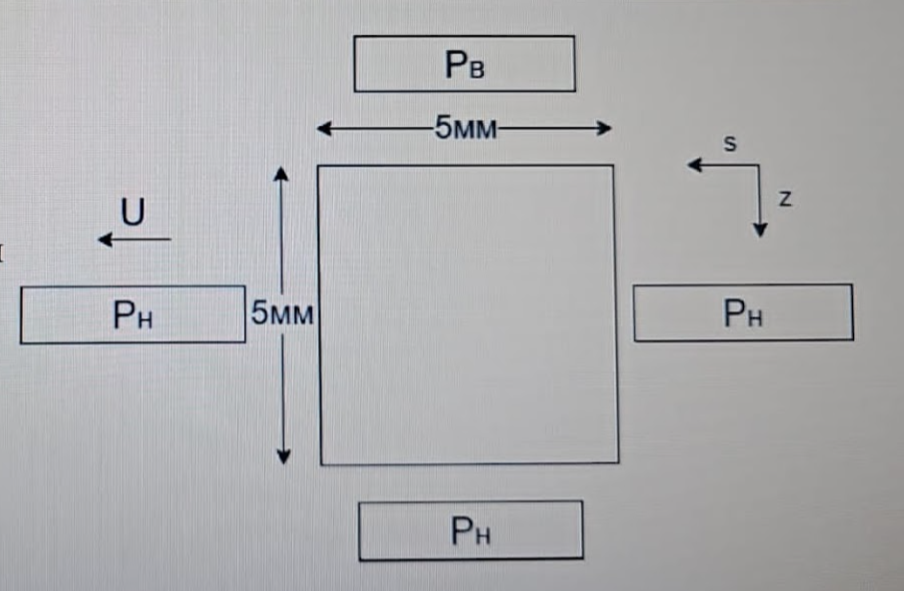
\includegraphics[width=0.4\textwidth]{taskGU}%
	\caption{Cхема области решения задачи}
	\vspace*{-2mm}
	\label{ser_graph}
\end{figure}
	
\end{frame}

\begin{frame}{}
	\begin{block}{}
	\[
	\int_{S_i} {[N] \left(\frac{\partial}{\partial x} \left(h^3 \frac{\partial p}{\partial x} \right) + \frac{\partial}{\partial z} \left(h^3 \frac{\partial p}{\partial z} \right) - 6 \mu U \frac{\partial h}{\partial x}\right) dx dz} = 0.
	\]
	\end{block}

\begin{block}{Рассмотрим сумму интегралов}
	\[
		\int_{S_i} {[N] \left(\frac{\partial}{\partial x} \left(h^3 \frac{\partial \phi}{\partial x} \right)\right) dx dz}
	+
	\int_{S_i} {[N] \left(\frac{\partial}{\partial z} \left(h^3 \frac{\partial \phi}{\partial z} \right)\right) dx dz} 
	-\]
	\[ -
	\int_{S_i} [N]\left(6 \mu U \frac{\partial h}{\partial x}\right) dx dz = 0.
	\]
\end{block}
	
	
\end{frame}

\begin{frame}{}
	\begin{block}{Интеграл по частям для $x$}
		\[
		K1_i = \int_{S_i} {[N] \left(\frac{\partial}{\partial x} \left(h^3 \frac{\partial \phi}{\partial x} \right)\right) dx dz} = [N]\frac{d \phi}{dx}\Biggr|_{S_i} - \int_{S_i} {\frac{d[N]}{dx} \left(h^3 \frac{\partial \phi}{\partial x} \right) dx dz}
		\]
	\end{block}

\begin{block}{Интеграл по частям для $z$}
	\[
	K2_i = \int_{S_i} {[N] \left(\frac{\partial}{\partial z} \left(h^3 \frac{\partial \phi}{\partial z} \right)\right) dx dz} = [N]\frac{d \phi}{dz}\Biggr|_{S_i} - \int_{S_i} {\frac{d[N]}{dz} \left(h^3 \frac{\partial \phi}{\partial z} \right) dx dz}
	\]
\end{block}

\begin{block} {Для правой части}
	\[
	F_i = \int_{S_i} [N]\left(6 \mu U \frac{\partial h}{\partial x}\right) dx dz.
	\]
\end{block}

\[
(K1_i + K2_i )\phi = F_i
\]
	
	
\end{frame}

\begin{frame}{Заключение}
	В ходе работы получены следующие результаты:
	\begin{block}{}
	\begin{enumerate}	
		\item Вывод уравнения Рейнольдса для установившегося течения в газовом смазочном слое.
		\item Было рассмотрено решение уравнение Рейнольдса с помощью метода конечных элементов.
	\end{enumerate}
	\end{block}	
\end{frame}	
\end{document} 